\subsection*{Groep IO}

Hieronder een overzicht van alle uitgevoerde bezigheden van deze week:

\begin{itemize}

\item
Een logo ontworpen voor het project \ref{fig:logo}

\item
Ontwerp van de inlogpagina \ref{fig:main} voor de mobiele user interface.

\item
Een nog niet uitgewerkt ontwerp van de toepassingen in de mobiele user interface \ref{fig:html_idee_1},\ref{fig:html_idee_2},\ref{fig:html_idee_3}

\item
HTML5 bronnenlijst op de server gezet \url{http://solarpoweredbikes.tudelft.nl/bronnen.html}

\item
HTML5 opzet met forms voor de inlogpagina

\item
Klein stukje CSS geschreven

\item
Geoefend met PHP en MySQL

\end{itemize}

\noindent
Hieronder een overzicht van alle bezigheden voor volgende week:

\begin{itemize}

\item
Authentificatie tussen de HTML5 inlogpagina en de PHP server

\item
HTTPS, vragen of dit mogelijk is

\item
Uitzoeken of cookies nodig zijn

\item
Uitwerken van de ontwerpen

\item
Globale indeling mobiele HTML pagina maken

\item
Gepersonaliseerde gegevens kunnen verzenden vanaf de PHP server



\end{itemize}

\begin{figure}[htbp]
\centering

\includegraphics[width=5cm]{images/logo.png}
\caption{Logo voor het Project SUNRISE}\label{fig:logo}
\end{figure}

\begin{figure}[htbp]
\centering
\includegraphics[width=10cm]{images/main.png}
\caption{Ontwerp voor de inlogpagina}\label{fig:main}
\end{figure}

\begin{figure}[htbp]
\centering
\includegraphics[width=15cm]{images/html_idee_1.jpg}
\caption{Ontwerp voor de app (reserveren)}\label{fig:html_idee_1}
\end{figure}

\begin{figure}[htbp]
\centering
\includegraphics[width=10cm]{images/html_idee_2.jpg}
\caption{Ontwerp voor de app (informatie oplaadstation)}\label{fig:html_idee_2}
\end{figure}

\begin{figure}[htbp]
\centering
\includegraphics[width=10cm]{images/html_idee_3.jpg}
\caption{Ontwerp voor de app (geschiedenis)}\label{fig:html_idee_3}
\end{figure}